\section{Experiment Design}

We designed the following experiment to compare the four NEAT
implementations described in the previous session in regards to their
victory ratio and survival ratio.

\subsection{Match Specification}

The experiment focuses on a matchup between a squad of units
controlled by the NEAT implementation, and a squad of units controlled
by the standard starcraft controller. Four unit matchups were defined:
\begin{enumerate}
    \item 22 marines vs 22 marines
    \item 22 marines vs 44 zerglings
    \item 22 vultures vs 22 vultures
    \item 22 vultures vs 22 zealots
\end{enumerate}

\begin{figure}
    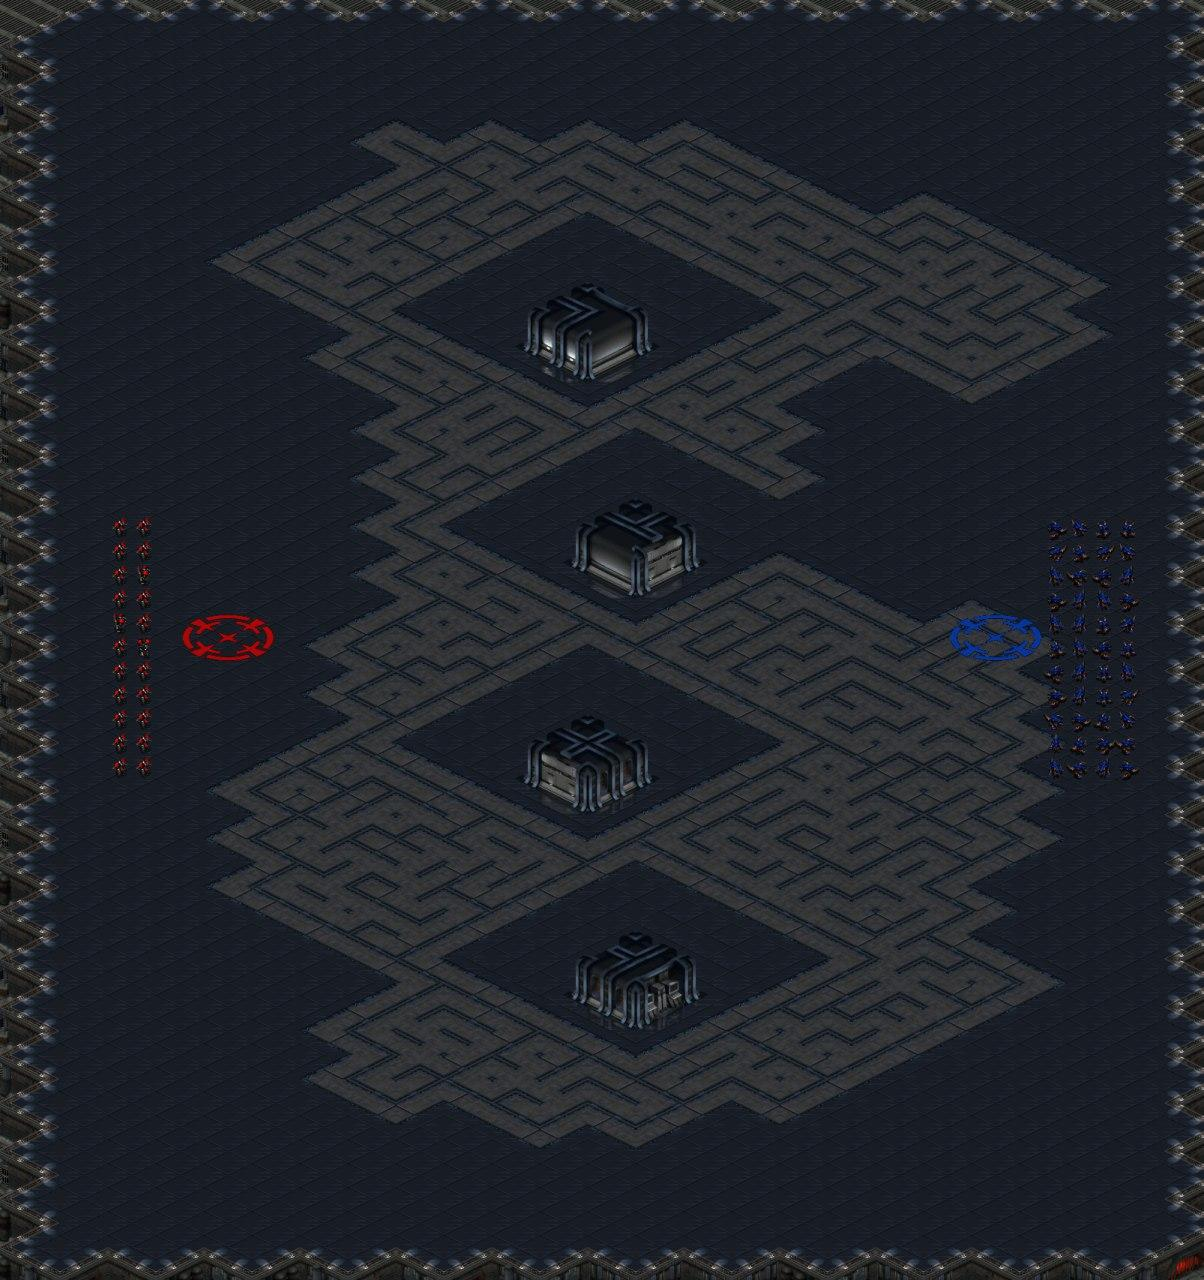
\includegraphics[width=.5\textwidth]{figures/scenario_map_overview}
    \caption{The map used for all matchups}\label{fig:map_overview}
\end{figure}

In these matchups, the marines have stimpacks, but no other upgrades
are added to the units. The match occurs in a custom map with four small obstacles
on the middle, and the units of both sides start at
opposite ends of the map as shown on Figure~\ref{fig:map_overview}.

The units matchup were chosen to see if the controller could learn a
kiting behavior that helps preserve units. Additionally, the case of
marines (matchups 1 and 2) has the additional problem of stimpack
usage: Using a stimpack damages the unit in exchange of a boost in
speed. This causes a deceptive problem where the usage of stimpack
causes a short term penalty in exchange of a possible longer term gain
in victory and survival ratios. In particular, the marine vs zerglings
matchup is very difficult to win without proper stimpack usage, so we
would expect the controllers to learn it.

\subsection{Learning and Comparison specification}

The comparison among techniques is composed of two stages: learning
and evaluation.

At the learning stage, we execute a complete evolution run with 100
generations for each combination of matchup and technique 3 times (for
a total of 48 evolution runs). The average fitness, best fitness and
number of survivors is logged for each generation.

After the learning stage, we evaluate each method by extracting the
five best genomes produced during the three evolution runs, and using
them for 50 games on an identical matchup. For these games, we log
the number of survivors and whether the game ended in victory or loss.

\subsection{Parameter Specifications}

Both the NEAT variants and the Starcraft Bot require multiple
parameters to be tuned in advance of any sort of experimentation. We
highlight some parameters that we feel are important for a better
understanding of the experimental results. A full list of the
parameters used can be obtained at the project github repository
listed in section~\ref{section:proposal}.

% IMPORTANT QUESTION: ARE WE USING A STANDARD NEAT LIBRARY? IF NOT,
% WHERE DO THE STANDARD NEAT PARAMETERS COME FROM?

\begin{tabular}{rll}
    \toprule
    Parameter & Value & Tweaks \\
    \midrule
    Number of inputs & 5 & 6 for marines \\
    Number of outputs & 4 & 5 for marines \\
    Initial population size & 22  & — \\[1ex]

    Compatibility threshold & 2 & — \\
    Dynamic compat. thresh. & true & — \\
    Target number of species & 4 & — \\
    Keep same species' representant & true & — \\[1ex]

    Use best genomes library & true & false if NS \\
    Bad genome max fitness & 100 & 1000 if Unified \\
    \bottomrule
\end{tabular}

The reason for overriding these parameters is as follows: The
\emph{initial population size} matches the number of controlled units
in the squad.  The \emph{number of inputs and outputs} for marines is
greater because the marine unit has to decide whether to use the
stimpack (output), and can sense whether the stimpack is ready for
activation (input). The \emph{keep same species' representant}
parameter is used to avoid the update of the representant of species
with a random member at each generation as described in the original
NEAT paper and instead keep the first representant of the species. The
best genomes library is not used for Novelty Search because NS does
not use the fitness as a performance metric. Instead, a separate list
of the best genomes is managed. The \emph{bad genome max fitness}
determine which genomes are to be considered bad given the
fitness. These genomes may occasionally be replaced by one from the
best genome library.

%The distance coefficients are used in the compatibility distance formula which is
%\[dist = c1 × \frac{E}{N} + c2 × \frac{D}{N} + c3 × W\]
%with N the number of genes of the larger genome, E the number of excess genes,
%D the number of disjoint genes and W the average weight differences of matching genes.
%The is the original compatibility distance formula.~\cite{StMi02}

Also, for the Cascade Neat variant, some mutation probabilities are modified:

\begin{tabular}{rl}
    \toprule
    Parameter & Value \\
    \midrule
    Add link & 0.00 \\
    Add neuron & 0.00 \\
    Remove neuron & 0.00 \\
    Add cascade & 0.03 \\
    Remove gene & 0.00 \\
    \bottomrule
\end{tabular}

These parameters were either taken from existing literature, or
obtained through experimentation.

{\bf TODO} cite sources for parameters values.

%%%%%%%%%%%%%%%%%%%%%%%%%%%%%%%%%%%%%%%%%%%%%%%%%%%%%%%%%%%%%%%%%%%%%%%%%%%%

Finally, we discuss the parameters for the NEAT starcraft bot:

\begin{tabular}{rl}
    \toprule
    Parameter & Value \\
    \midrule
    Frames per update & 10 \\
    Max distance NN & 1500 \\
    Max entities NN  & 20 \\[1ex]

    Survival perf weight & 0.5 \\
    Attack perf weight  & 0.5 \\
    Cooperative perf weight & 10 \\
    Unified attack perf weight & 0.33 \\
    Unified cooperative perf weight & 100 \\
    Exponent on fitness & 1.3 \\
    \bottomrule
\end{tabular}

``Max distance NN'' and ``Max entities NN'' are, respectively, the
maximal distance and the maximal number of entities a neural network
can perceive.  This is used for normalization purposes. All values
greater than these will result in the value \(1\) being fed as the
input so that all inputs are in range \([0, 1]\).

\subsection{Fitness Specification}

The weights are used to model the fitness function. There are two
fitness functions, according to whether the Unified NEAT variant is
being used or not.  The regular fitness function is given by
\begin{equation*}
  (\text{damages\_dealt} \times A + \text{health} \times B + \text{survivors} \times C)^D,
\end{equation*}
while the fitness for the Unified NEAT variant is
\begin{equation*}
  (\text{damages\_dealt} \times A + \text{survivors} \times C)^D.
\end{equation*}
Here \emph{A} is the attack performance weight, \emph{B} the survival
performance weight, C is the cooperative performance weight and D is
the exponent on the fitness.

To encourage the variants to find strategies that promote cooperation
and survival, we have included the number of survivors as a component
of the fitness function.
